\documentclass[10pt,letterpaper]{article}

\usepackage{latexsym}
\usepackage{fancybox}
\usepackage{graphicx}
\usepackage{soul}
\usepackage{amssymb}
\usepackage{color}
\usepackage{ulem}
\usepackage{float}
\usepackage{xspace}
\usepackage{graphics}
%\usepackage{rotating}
\usepackage{setspace}
\usepackage{multirow}
\usepackage[abs]{overpic}
\usepackage{url}
\usepackage[font=scriptsize,labelfont=bf]{caption}
\usepackage{enumitem}
\usepackage{wrapfig}
\usepackage{tabu}
\usepackage{pgfgantt}

\usepackage{natbib}
\setlength{\bibsep}{0pt}
\citestyle{plain}


\input{defs}
%\newcommand{\annrev}{ARA\&A}
\newcommand{\apj}{ApJ}%% Journal abbreviations
\newcommand{\apjs}{ApJS}
\newcommand{\apjl}{ApJL}
\newcommand{\aap}{A{\&}A}
\newcommand{\aaps}{A{\&}AS}
\newcommand{\mnras}{MNRAS}
\newcommand{\aj}{AJ}
\newcommand{\araa}{ARAA}
\newcommand{\pasp}{PASP}
\newcommand{\nat}{Nature}
\newcommand{\procspie}{Proc. of SPIE}

\pretolerance=10000
\textwidth=7.25in
\textheight=9.9in
\voffset = -0.7in
\topmargin=0.0in
\headheight=-0.1in
\hoffset = -0.3in
\headsep=0.4in
\oddsidemargin=0in
\evensidemargin=0in
\parindent=1.2em
\parskip=0.1ex

\newcommand{\sqdeg}{\ensuremath{\mathrm{deg}^2}}
\newcommand{\sqarcmin}{\ensuremath{\mathrm{arcmin}^2}}
\newcommand{\nm}{\ensuremath{\mathrm{nm}}}
\newcommand{\ang}{\ensuremath{\mathrm{\AA}}}
\newcommand{\mpc}{\ensuremath{h^{-1}\,\mathrm{Mpc}}}
\newcommand{\micron}{\ensuremath{\mu\mathrm{m}}}
\newcommand{\texp}{\ensuremath{t_\mathrm{exp}}}

\begin{document}

\pagestyle{myheadings}    % Go for customized headings
\markboth{\hfill \footnotesize 2017 Keck Instrumentation White Paper: Fiber-Fed MOS for Keck \hfill}{\hfill \footnotesize 2017 Keck Instrumentation White Paper: Fiber-Fed MOS for Keck  \hfill}
\vspace*{-0.3in}
\noindent
%\doublespacing
\begin{centering}
%\large \textit{2016 Keck Instrumentation White Paper} \\
\Large \textbf{FOBOS: A Fiber-Fed MOS for Keck} \\
\end{centering}

\vspace{0.5em}
\noindent
\begin{centering} \small
David Schlegel\footnotemark[1] (LBNL), Khee-Gan Lee\footnotemark[1] (LBNL), Kevin Bundy (UCSC/UCO),
R.~Michael Rich (UCLA),  
Connie Rockosi (UCSC/UCO), Dan Weisz (UCB), J.~Xavier Prochaska (UCSC/UCO)
 %A. Coil (UCSD),  A. Kim (LBNL), 
%Joseph Hennawi (UCSB), \\ M.\ Kriek (UCB), D.\ Weisz (UCB),
%K. Bundy (UCO), A.\ Leauthaud (UCSC), M.\ Cooper (UCI)
\vskip 0.5em
\textit{Draft, June 7th 2017} \\
\end{centering}

\footnotetext[1]{E-mails: \textit{djschlegel@lbl.gov}; \textit{kglee@lbl.gov}}
\addtocounter{footnote}{1}
\vspace{-1em}
\subsection*{Project Justification}
The 2016 Keck Strategic Science Plan (SSP) has called
for Keck's strengths in faint multiplexed spectroscopy to be maintained and enhanced through the next decade.
In particular, WMKO is in pole position to provide unique deep spectroscopic capability in the NUV/blue ($\lambda<400$nm) 
to complement JWST, 
 while an enhanced multiplexing will enable efficient follow up of objects identified by upcoming imaging
 surveys such as LSST, Euclid, and WFIRST. 
While the SSP suggested achieving these capabilities with a DEIMOS upgrade with a second focal plane 
 and/or a blue spectral channel, recent advances in fiber spectroscopy and sky subtraction now allow these capabilities to be achieved ---
and indeed
significantly surpassed --- by building a fiber MOS.
We therefore propose the Keck Fiber-Optic Broadband Optical Spectrograph (FOBOS), a 500-object
fiber-fed spectrometer sampling the full Keck focal plane, providing medium resolution ($R\sim 2500-5000$) spectroscopy over 
a large optical range (350-980nm).


 Crucially, the importance of massively-multiplexed optical spectroscopy on a 8-10m class telescope
  has been recognized at the national level
 by both the NSF \cite{najita:2016} and DOE \cite{dodelson:2016}. 
While multiple concepts are now starting to be proposed for various US facilities,
it is unlikely that any of these can get on-sky before the mid-2020s.
 Keck-FOBOS, on the other hand, leverages the sigificant R\&D of the upcoming DESI project and 
 could begin operations near the start of 
 LSST and Euclid science operations in $\sim 2022$. This makes it a strong contender for national funding for
 its overall \$12-15M cost (including contingency and overheads), 
 but \emph{we request \$35k in funding from WMKO to continue our feasibility studies and begin building a case for external funding}.
 
 \vskip0.2em
\noindent{\bf Baseline Concept:} FOBOS will be a Nasmyth instrument on one of the Keck telescopes,
with 500 robotic fiber positioners and mini-IFUs at the focal plane coupling to in-situ spectrographs based on the 
DESI design\footnote{Currently being built for the 4m Mayall on Kitt Peak.}.
The spectrograph units are designed for high throughput ($\sim 70\%$, see Fig.~\ref{fig:spectrographs}) over three spectral channels: 
blue ($\lambda=350\nm-560\nm$ at $R\sim2500$),
red ($\lambda=560\nm-750\nm$ at $R\sim 4000$) and NIR ($\lambda=750\nm-980\nm$ at $R\sim 5000$).
\begin{wrapfigure}{l}{0.35\textwidth}\footnotesize 
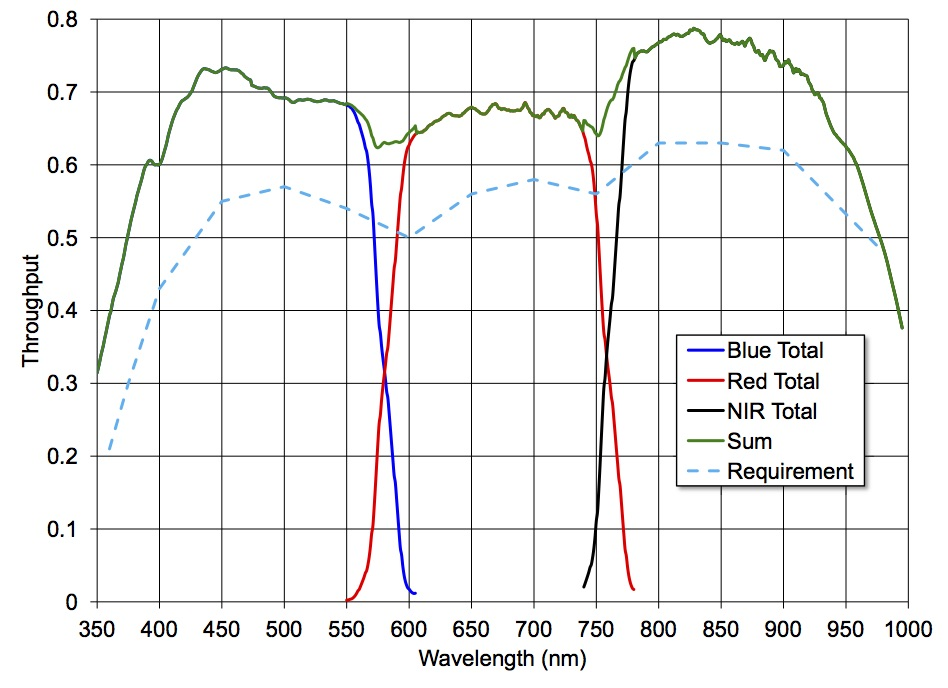
\includegraphics[width=0.35\textwidth]{throughput.jpg}
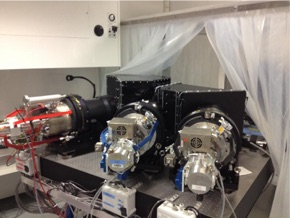
\includegraphics[width=0.34\textwidth]{desispec_unit0.jpg}
\caption{\label{fig:spectrographs}
(Top) Design throughputs for the DESI spectrographs, showing the individual spectral channels
as well as combined throughput.
(Bottom) Photograph of the first DESI spectrograph unit, which was completed in fall 2016 and is
currently undergoing testing at Marseille. The overall performance has so far been found to be nominal.
}
\end{wrapfigure}
We envision the entire FOBOS instrument fitting on the Nasmyth position with
a footprint smaller than DEIMOS, where the fiber focal plane+rotator is coupled to the bench-mounted
spectrographs via a short fiber run of several meters. This reduces fiber throughput losses while providing the stability of a fixed
gravity vector for the spectrographs.
We have been in touch with M.\ Kassis (WMKO) regarding space/weight constraints, and have confirmed that the 
full focal plane/spectrograph assembly would fit in one of the Keck Nasmyth slots.
The exact location will depend on the WMKO instrumentation plan for the next decade; options include
awaiting the retirement of HIRES after KPF becomes operational, 
decommissioning DEIMOS, or possibly extending the K2 Nasmyth deck to create a new instrument slot.

The DESI design uses 107$\mu$m fibers that need to be injected at $f$/3.9, which translates to
a $0.57''$ aperture once matched to the Keck $f$/15 focal plane with microlenses.
This would likely be too small for individual fibers, so we will instead combine them into mini-IFUs
comprised of $7\times0.57''$
hexagonal microlens arrays for each target.
The signal from all 7 fibers on each target
can be optimally-combined to yield superior S/N and maximize flexibility
across all seeing conditions: in good seeing, 
most of the flux goes through the central fiber with reduced sky background,
while in bad seeing the overall $1.71"$ footprint help capture the extended flux. 
The small size of the individual $0.57"$ fibers also means FOBOS would be able to take advantage of 
ground-layer AO if it is implemented on Keck in the future. 
The microlens arrays are the critical R\&D item since they underpin the feasibility of the whole project, 
and thanks to a Mini Grant from UCO we have been able to begin preliminary optical design on the microlens
but require more funding to complete this study.

\vskip0.2em
\noindent{\bf FOBOS in Context:}
FOBOS will be a powerful and flexible instrument --- equally
suited for both PI-led science and surveys
--- that will maintain Keck's proven strength in faint multiplexed spectroscopy established by LRIS, DEIMOS, and MOSFIRE.
A natural comparison arises with Subaru-PFS \cite{sugai:2015}, with its ultra-wide FOV (1.3 deg$^2$) and huge multiplexing (2400).
While FOBOS will concede the overall FOV and multiplexing advantage, it will be optimized to
observe faint objects, with $2\times$ better
system throughput than PFS and $1.5\times$ greater telescope collecting area, while the mini-IFUs confer $20\%$ higher S/N,
at $0.6''$ seeing,
over PFS's $1.1''$ fibers, equivalent to $1.4\times$ throughput gain.
These factors combine into a $4\times$ speed advantage,
\emph{allowing FOBOS to access sources $\sim1$ mag fainter than PFS},  
thus enabling a complementary set of science goals that will lie beyond the reach of PFS.
%These factors combine to imply that FOBOS requires $\sim 4\times$ shorter exposure times than PFS
%at fixed magnitude and S/N, which
 %makes up for the lower multiplexing and grants FOBOS an overall spectroscopic efficiency 
 %roughly comparable to PFS for science cases that do 
%not require ultra-wide FOV. 
%FOBOS also has $\sim 50\%$ better resolution than PFS.
%At first light, FOBOS will not push as far into the NIR as PFS (980nm vs 1.3\micron) but will have superior NUV coverage
%(350nm vs 400nm), and our team is looking into a redesign of the spectrograph baffles and slitheads to accommodate future upgrades to
 %a fourth $1-1.2\micron$ spectral arm, possibly
 %using Ge-based CCDs currently under development (see, e.g., \cite{dodelson:2016a}). 

\begin{wrapfigure}{r}{0.5\textwidth}\footnotesize
\captionof{table}{Summary of Wide-Field Spectroscopic Options for Keck} \label{tab:comparison} 
\begin{tabu}{l | c | c |c}
%\caption{\label{tab:instr} Keck Spectroscopic Upgrade Options}
\multirow{2}{*}{Instrument} & \multirow{2}{*}{FOBOS} & \multirow{2}{*}{DEIMOS} & DEIMOS \\
  &  &  &  (2$\times$ focal plane) \\
  \hline
  Multiplex  & 500 & 125 & 250 \\
  Max targets/night &  $\sim$30000 & 1250 & 2500 \\
FOV (arcmin$^2$) & $\sim 300$ & 84  & 168  \\
Spectral length, $\Delta \lambda$ (nm) & 620 & 260-530 & 260-530 \\
Resolution FWHM ($\ang$)  & 1.75 & 1.1-3.5 & 1.1-3.5
%\enddata
\end{tabu}
\end{wrapfigure}

Last year's SSC comments requested that we compare FOBOS with possible upgrades
of DEIMOS. 
On paper, FOBOS is clearly superior to an upgraded DEIMOS with a second focal plane (summarized in Table~\ref{tab:comparison}).
FOBOS's overall FOV would be $\sim 1.8\times$ that of upgraded DEIMOS and would have double the
multiplexing. 
The fibers can be rapidly repositioned ($<1$ min) making feasible programs with short ($<$10 min) 
exposures that are impractical with DEIMOS, which can only load 10 slitmasks per night. 
Even if DEIMOS can be upgraded with a LRIS-like blue spectral channel, which we consider unlikely, 
it could only offer resolutions comparable to FOBOS 
($R\sim 2500-5000$ from blue to red) over limited wavelength ranges and discontinuous coverage.
The only remaining question was whether sky subtraction on fibers work well enough
 to manifest these advantages. With the kind permission of the OzDES collaboration \cite{yuan:2015}, we have analyzed the
 performance data from their deep fiber spectroscopy of $r>24$ galaxies, to forecast the performance of an analogous 
 instrument on Keck. We find that \emph{the S/N-exposure time scaling for fibers should behave roughly Poisson-limited up to 
 $\texp < 3-4$hrs on Keck}, and indeed 
 shows some throughput advantage compared to slits. 
 With longer exposure times, the fiber S/N improves more slowly than the ideal scaling, 
 but the multiplex advantage makes up for this over upgraded DEIMOS. 
 It is only if very long exposures are required ($\texp>15$hrs) are required that upgraded DEIMOS
 holds the advantage, and even this assumes perfect sky subtraction for slits --- which is not certain. 
This study is
 appended to the end of this White Paper for the SSC's perusal, but we emphasize that this forecast 
 assumes only existing fiber reduction techniques. For long-exposure programs, 
 it is likely that a nod-and-shuffle observing mode
 could allow near-perfect sky subtraction at the cost of some multiplexing. It might also be possible to
  leverage the latest innovations developed for fiber-fed high-resolution spectrographs, 
  such as fiber scramblers or octagonal fibers, to mitigate the PSF variations that lead to sky subtraction errors. 
  
Finally, at the time of writing TMT/WFOS is considering
fibers to achieve its design goals, with ongoing work to define a fiber reference design in preparation for a downselect 
in early 2018. This is thus a time-limited opportunity for shared R\&D between WFOS and FOBOS
especially since WFOS PI K.\ Bundy is part of our team.
The WFOS team will consider innovations
that will allow ultra-faint spectroscopy with fibers on TMT, and our teams will work together to exploit the clear
synergy between the two projects.


 \vskip0.2em
\noindent{\bf Cost and Risk:} The DESI project is now undergoing construction, and therefore the costs are well known. The contracted build cost for the spectrographs (with WinLight, France) is $\$1.5$M per unit including testing and validation labor costs, 
of which FOBOS would require 4 units. While the cost might change slightly for FOBOS since a new contract would
need to be negotiated, the FOBOS spectrographs provides a well-understood cost baseline 
of $\sim\$6$M-$\$7$M along with minimal technical risk.

In DESI, the focal plane array costs $\sim \$1$k per fiber+positioner (including electronics and mechanicals), 
so we conservatively estimate
\$3.5k per mini-IFU+positioner combination, costing $\sim $\$1.8M for the full focal plane array.
Our concept includes an ADC to enable simultaneous blue-red observations, which can be of similar
design as the K1 Cass ADC \cite{phillips:2006} and should be a straightforward implementation 
costing $\sim \$1.5$M. \emph{We thus estimate $\sim\$10$M in hardware costs, translating to a $\sim\$12-\$15$M
full project cost including R\&D, overheads, and contingency.} 

Another attractive aspect of the FOBOS concept is its modularity, which allows
early on-sky testing and phased commissioning to reduce risk. For example, the DESI project benefitted tremendously from the
``Proto-DESI'' demonstrator, a low-cost (\$XX) on-sky test of the DESI guide cameras and a few
robotic positioners which retired the risk in these systems before integration into the full instrument. 
FOBOS could also begin operations at partial scope: even with half of its positioners, fibers, and spectrographs, 
it would already be superior to DEIMOS. This could, for example, allow us to pursue funding in stages rather than
seeking the full project cost from the outset.

\clearpage

 \subsection*{Budget Request} 
\emph{We request \$35k in WMKO funding to complete the feasibility study on the FOBOS microlens arrays}, which is the critical
system to couple the Keck focal plane with the DESI fiber and spectrograph systems.
The study will aim to design $7\times 1$ hexagonal microlens arrays that will couple the Keck $f$/15 focal plane
to mini fiber-bundles at the $f$/3.9 speed required for injection into the DESI fiber system. 

We began this study several months ago with UCO funding, and have been examining modifications of the 
GMOS IFU epoxy/fused silica microlens arrays to couple Keck with DESI. By the start of WMKO funding in Oct 2017, we expect
to have preliminary optical designs in hand, and will begin optimizing the coatings and materials in order to maximize performance, 
as well as designing the ferrules that will bond to mini-fiber bundles.
This will require liaising with possible vendors and obtaining samples for testing.

The cost breakdown for the project is as follows:

\begin{enumerate}[label=(\textit{\roman*})]
	\item {\bf Optical Engineer Time at 0.4FTE $\times$ 12 weeks, \$20k}. Tim Miller (UCB/SSL) will continue his work on the
	microlens design for FOBOS, which was begun this year with support from UCO. He can only provide partial effort due to 
	other commitments to the DESI and Keck/KPF projects.
	\item {\bf Microlens Sample Acquisition and Testing, \$10k}. This will allow us to acquire samples for microlens 
	arrays based on our optical design, and carry out optical testing to verify the throughput and PSF performance.
	\item {\bf Optical Fibers and Ferrules, \$5k}. For acquiring the fibers and ferrules to physically couple with the microlens arrays, 
	needed to test the optical performance of the former.
\end{enumerate}

\subsection*{Project Timeline}
Our medium-term goal is to demonstrate feasibility in order to apply for a $\sim\$300$k NSF ATI grant in November 2018, 
to fund the full instrument design prior
to a NSF MSIP application for the full project funding. The following is the strawman project timeline over the next 1.5 yrs:

\vspace{1em}
\begin{ganttchart}[
hgrid,
vgrid,
newline shortcut=true,
time slot format=isodate-yearmonth,
compress calendar,
bar label node/.append style=%
{align=left}
]{2017-04}{2018-11} \baselineskip0.1em
\gantttitlecalendar{year, month} \\
\ganttbar{\scriptsize Preliminary Microlens Design \ganttalignnewline \scriptsize (UCO-funded)}{2017-04}{2017-09} \\
\ganttlinkedbar{\scriptsize Microlens Design \& Testing \ganttalignnewline \scriptsize(WMKO-funded)}{2017-10}{2018-02} \ganttnewline
\ganttbar{\scriptsize Collaboration with TMT/WFOS team\ganttalignnewline \scriptsize on WFOS Fiber Reference Design}{2017-07}{2018-04} \\
\ganttmilestone{\scriptsize UCO Mini-Grant Application}{2017-10} \\
\ganttbar{\scriptsize ADC \& Fiber Positioner Design \ganttalignnewline \scriptsize (UCO-funded)}{2017-12}{2018-09} \\
\ganttmilestone{\scriptsize NSF ATI Submission Deadline}{2018-10}
\end{ganttchart}


{
\bibliographystyle{apj}
\bibliography{apj-jour,lyaf_kg,lss_galaxies,my_papers}
}
 
\end{document}
